
%(BEGIN_QUESTION)
% Copyright 2011, Tony R. Kuphaldt, released under the Creative Commons Attribution License (v 1.0)
% This means you may do almost anything with this work of mine, so long as you give me proper credit

A FOUNDATION Fieldbus pressure transmitter is used to sense the mass of liquid stored inside a cylindrical vessel having a diameter of 70 inches and a height of 115 inches.  The liquid's density is 54 pounds per cubic foot (equivalent to 86.5\% the density of water):

$$\includegraphics[width=15.5cm]{i03646x01.eps}$$

Determine the proper {\tt XD\_Scale}, {\tt OUT\_Scale}, and {\tt L\_Type} parameter values to make the transmitter functional over the entire height of the tank.

\underbar{file i03646}
%(END_QUESTION)





%(BEGIN_ANSWER)

{\tt XD\_Scale} = 0 to 99.47 inches of water

\vskip 10pt

{\tt OUT\_Scale} = 0 to 13,830.4 pounds

\vskip 10pt

{\tt L\_Type} = Indirect

\vskip 10pt

Hint: with a density 86.5\% that of water, a full tank (115 inches) will generate 86.5\% as much pressure as if it were filled with water.  This is why a height of 115 inches only generates 99.47 inches of water pressure.

%(END_ANSWER)





%(BEGIN_NOTES)


%INDEX% Fieldbus, instrument ranging: setting XD_Scale and OUT_Scale parameters for an application

%(END_NOTES)


